% ===== 底本 第 3 章《环簇 Fano 集的 SYZ 镜像对称》；片段 tr03a；源块 B105--B115 =====

\section{环簇 Fano 集的 SYZ 镜像对称}

% [源 B105]
本讲讨论拉格朗日纤维化的第一类非正则奇点，我们称之为\emph{环面奇点}（toric singularities）。这类奇点之所以好，是因为来自拉格朗日环面纤维化的环面作用可以延拓到奇异纤维上，且在这些纤维上稳定化子群非平凡。最简单的情形之一便是所谓的\emph{环簇}（toric varieties）：此时底空间 $B$ 的正则层就是 $\mathbb{R}^n$，而我们很快会看到，奇点层构成一个部分紧化 $\mathbb{R}^n$ 的多面体复形。

% [Tutor Note: B105 的 stabilization groups 即 stabilizer groups（稳定化子群），与 B111 的 "stabilizer subgroups" 是同一概念；原文用词不同，译文按语义统一作「稳定化子群」，未改动原文的其他内容。]

% [源 B106]
\subsection{辛环簇}

% [源 B107]
本节我们以辛几何的方式回顾环簇的定义，以便记录其辛（Kähler）结构。

% [源 B108]
\begin{definition*}
一个\emph{辛环簇流形}（symplectic toric manifold）$(M,\omega)$ 是指一个辛流形连同其上的哈密顿 $\mathbb{T}^n$-作用。
\end{definition*}

% [源 B109]
$M$ 上的哈密顿 $G$-作用诱导李代数同态 $\rho\colon\mathfrak{g}\to C^{\infty} (M)/\mathbb{R}$，等价地，诱导一个在 $\mathfrak{g}^{\ast}$ 中相差一个平移的意义下确定的映射 $\mu_G\colon M\to\mathfrak{g}^{\ast}$，其中 $\mu_G(x)(X):=\rho (X)(x)$；该映射称为 $G$ 的\emph{矩映射}（moment map）。当 $G=\mathbb{T}^n$ 是环面时，Atiyah--Guillemin--Sternberg 定理 [Ati82, GS82] 断言

% [源 B110]
\begin{theorem*}[Atiyah--Guillemin--Sternberg]
$\mu_G\colon M\to\mathfrak{g}^{\ast}$ 的像是凸多面体。
\end{theorem*}

% [源 B111]
我们把矩映射的像称为辛环簇流形 $M$ 的\emph{矩多面体}（moment polytope）。设 $\Sigma$ 是 $\mathfrak{g}^{\ast}$ 中的多面体，它自然带有按面（facet）的分层。只有一个最高维的面 $\Sigma^{\circ}$，它对应那些使 $T^n$ 在纤维上自由传递地作用的 $\mu_G$ 值，而这些纤维正是 $M$ 中的拉格朗日环面。低维的面则对应那些使 $T^n$ 的作用具有稳定化子群的 $\mu_G$ 值，稳定化子群的秩等于相应面的余维数。它们自然是迷向环面，阻碍纤维化成为正则的。

% [Tutor Note: B111 把 $\mathfrak{g}^{\ast}$ 中的多面体记作 $\Sigma$，而 B113/B115 又用同一个 $\Sigma$ 表示扇；这是原文在两个语境里复用同一符号（并非笔误），转写时一律保留 $\Sigma$，不要擅自改成 $P$。]

% [源 B112]
\begin{figure}[htbp]
\centering
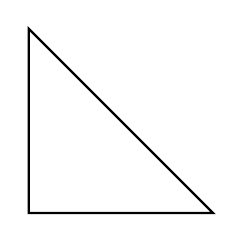
\begin{tikzpicture}[scale=0.9]
  \draw[thick] (0,0) -- (0,2.6) -- (2.6,0) -- cycle;
\end{tikzpicture}
\figtitle{1}{$\mathbb{P}^2$ 的矩多面体。}
\end{figure}
\begin{example*}
下面用一个简单的例子说明如何从矩多面体读出环簇的几何信息。考虑具有标准辛结构的辛向量空间 $\mathbb{C}^3=\mathbb{R}^6$，其上有标准线性作用 $T^3\curvearrowright\mathbb{C}^3$：$(t_1, t_2, t_3).(x,y,z):=(t_1 x,t_2y,t_3z)$。$\mathbb{P}^2$ 可以通过 $\mathbb{R}^6$ 对对角环面作用 $(x,y,z)\mapsto (tx,ty,tz)$ 的\emph{辛约化}（symplectic reduction）得到，其中要选取正则参数 $\lambda\in (0,\infty)\subseteq\mathfrak{t}=\operatorname{Lie} (\mathbb{T}^1)$。矩映射 $\mu_{\mathbb{T}^3}$ 用标准基可以显式写成
\[
  \mu_{\mathbb{T}^3} (x,y,z)=\frac{1}{2} (|x|^2,|y|^2,|z|^2),
\]
于是用前两个坐标，就可以把 $\mathbb{P}^2$ 上诱导的矩映射 $\mu_{T}$ 写成
\[
  \mu_{T} ([x:y:z])=\left(\frac{|x|^2}{2},\frac{|y|^2}{2}\right).
\]
显然 $\mu_T$ 的像是三角形 $\{t_1\leq\sqrt{\lambda},\ t_2\leq\sqrt{\lambda},\ t_1+t_2\leq\sqrt{\lambda}\}$，如图 1 所示。矩多面体中的边 $\{t_1=0\}$ 对应除子 $\{x=0\}\subseteq\mathbb{P}^2$，在这条边上可以看到第一个圆周的作用是平凡的。类似地，另外两条边对应 $\mathbb{P}^2$ 的另外两个不动除子。同样容易看出，多面体顶点处的纤维是点，它们是环面作用的不动点。
\end{example*}

% [Tutor Note: B112 源文开头是底本用 canvas 画出的一幅三角形图（图题为 "Moment polytope for $\mathbb{P}^2$"），底本无位图可提取；本译本按其 canvas 绘制指令（三点 (0,√λ)、(√λ,0) 与直角顶点）用 tikz 重画为图 1，未改动任何数学内容。]

% [Tutor Note: B112 的三角形界 $\sqrt{\lambda}$ 与同段显式矩映射 $\mu_{\mathbb{T}^3}=\frac{1}{2} (|x|^2,|y|^2,|z|^2)$ 不自洽：令 $t_i=\frac{1}{2}|x_i|^2$，对角约化层取 $\lambda$ 时 $t_1+t_2+t_3=\lambda$，故 $\mu_T$ 的像应为 $\{t_1\geq0,\ t_2\geq0,\ t_1+t_2\leq\lambda\}$，直角边长为 $\lambda$，而非 $\sqrt{\lambda}$；若要直角边长为 $\sqrt{\lambda}$，须把约化层取成 $\sqrt{\lambda}$。此处照原文排印、未改数学，已登记 README。]

% [源 B113]
\begin{remark*}
代数几何学家大概更熟悉\emph{扇描述}（fan description）：簇 $X$ 上的代数 $\mathbb{G}_m^n$-作用给出 $\mathbb{R}^n$ 中一族锥的并，其中原点对应稠密环面轨道，射线对应除子，而高维锥对应高余维的环簇子簇。这两种图像在如下组合关系下大致等价：对给定的 $\mathbb{R}^n$ 中的扇 $\Sigma$ 与选定的向量 $(\lambda_i)\in\mathbb{R}^n$，可考虑多面体
\[
  P=\{x\in\mathbb{R}^n\vert \langle x,v_i\rangle\geq -\lambda_i,\ v_i\text{ 是 }\Sigma\text{ 中射线的生成元}\}
\]
于是 $(\lambda_i)$ 的选取就在环簇 $X$ 上给出一个与代数结构相容的辛结构。
\end{remark*}

% [源 B114]
现在我们转向环簇的 Fano 性。回忆一个辛流形是\emph{单调的}（monotone）或 \emph{Fano} 的，如果存在正常数 $\tau$ 使得 $[\omega]=\tau c_1 (X)$，其中 $c_1 (X)$ 是 $X$ 的第一 Chern 类。由于 $c_1 (X)$ 是整的，且在代数几何上等于出现在边界层上的所有环簇除子的代表类之和，于是 Fano 条件可以组合地读出如下：

% [源 B115]
\begin{definition*}[Batyrev；原文标为 Definition/Proposition]
环簇 $X$ 是 Fano 的，当且仅当与 $X$ 相伴的标准矩多面体 $P$ 是\emph{自反的}（reflexive）。设 $\Sigma$ 是 $X$ 的扇，定义
\[
  P=\{x\in\mathbb{R}^n\vert \langle x,v_i\rangle\geq -1,\ v_i\text{ 是 }\Sigma\text{ 中射线的生成元}\}
\]
为 $X$ 的标准矩多面体，则称 $P$ 是\emph{自反的}，如果它的\emph{极对偶}（polar dual）
\[
  P^{\circ}=\{y\in\mathbb{R}^n\vert \langle x,y\rangle\geq -1,\ \forall x\in P\}
\]
是整向量的凸包。
\end{definition*}

% [Tutor Note: B115 的自反性可用最小例子核验：取 $n=1$、扇的射线生成元为 $\pm 1$，则 $P=\{x\in\mathbb{R}\vert \pm x\geq -1\}=[-1,1]$，其极对偶 $P^{\circ}=[-1,1]$ 恰为整向量的凸包，故 $[-1,1]$ 自反（对应 $\mathbb{P}^1$ 为 Fano）；这可作为检验定义中各符号约定的一维锚点。]
